\documentclass[11pt]{article}
\usepackage{amsmath}
\usepackage{amssymb}
\usepackage{tikz}
\usepackage{geometry}
\usepackage{booktabs}
\geometry{margin=1in}

\title{Collaborative Filtering with Matrix Factorization:\\Book Recommendation System}
\author{Hardcover Book Friend Finder}
\date{\today}

\begin{document}

\maketitle

\begin{abstract}
We present a hybrid book recommendation system using collaborative filtering with matrix factorization. The model decomposes a sparse user-book interaction matrix into two lower-dimensional matrices representing latent features. We employ masking to handle extreme sparsity (95.75\%) and combine collaborative filtering with popularity-based recommendations to achieve 8.83\% precision@10, outperforming pure collaborative filtering by 308\%.
\end{abstract}

\section{Matrix Factorization}

\subsection{Problem Setup}

Given a user-book interaction matrix $Y \in \mathbb{R}^{m \times n}$ where:
\begin{itemize}
    \item $m$ = number of books (2,547)
    \item $n$ = number of users (246)
    \item $Y_{ij}$ represents user $j$'s interaction with book $i$
\end{itemize}

The matrix is highly sparse: only 26,598 interactions out of 626,562 possible (95.75\% sparse).

\subsection{Data Filtering}

From the raw dataset of 1,000 users and 45,203 books, we applied filtering to improve model quality:

\begin{itemize}
    \item \textbf{User filter}: Keep only users with $\geq 20$ book interactions (246 users retained, 24.6\%)
    \item \textbf{Book filter}: Keep only books with $\geq 5$ users (2,547 books retained, 5.6\%)
\end{itemize}

This reduces noise from inactive users and obscure books while maintaining sufficient data for collaborative filtering. The filtered dataset provides better signal for learning user preferences.

\subsection{Matrix Decomposition}

We factor $Y$ into two rectangular matrices:

\begin{equation}
Y \approx \sigma(X W^T + b)
\end{equation}

where:
\begin{itemize}
    \item $X \in \mathbb{R}^{m \times k}$ is the \textbf{book feature matrix} (2,547 $\times$ 20)
    \item $W \in \mathbb{R}^{n \times k}$ is the \textbf{user feature matrix} (246 $\times$ 20)
    \item $b \in \mathbb{R}^{1 \times n}$ is the user bias vector
    \item $k$ = 20 latent features
    \item $\sigma$ is the sigmoid activation function
\end{itemize}

\begin{center}
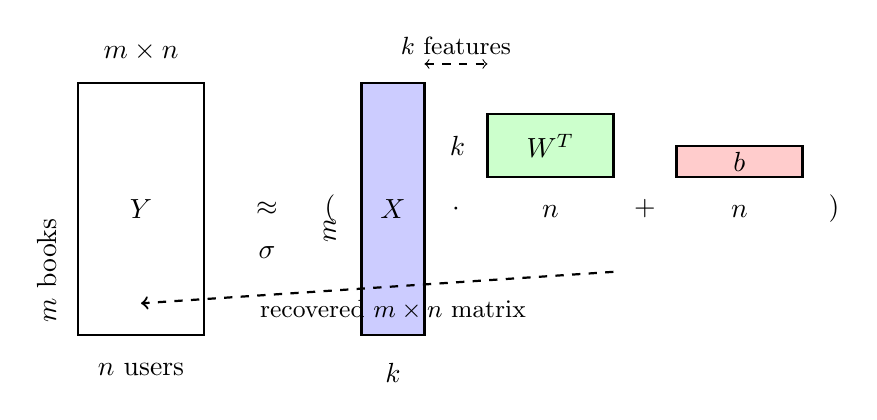
\begin{tikzpicture}[scale=0.8]
    % Y matrix
    \draw[thick] (0,0) rectangle (2,4);
    \node at (1,2) {$Y$};
    \node[below] at (1,-0.3) {$n$ users};
    \node[left,rotate=90] at (-0.5,2) {$m$ books};
    \node at (1,4.5) {$m \times n$};

    % Approximately equal
    \node at (3,2) {$\approx$};
    \node at (3,1.3) {$\sigma$};

    % Opening parenthesis
    \node at (4,2) {$($};

    % X matrix
    \draw[thick,fill=blue!20] (4.5,0) rectangle (5.5,4);
    \node at (5,2) {$X$};
    \node[below] at (5,-0.3) {$k$};
    \node[left,rotate=90] at (4,2) {$m$};

    % Multiplication dot
    \node at (6,2) {$\cdot$};

    % W^T matrix
    \draw[thick,fill=green!20] (6.5,2.5) rectangle (8.5,3.5);
    \node at (7.5,3) {$W^T$};
    \node[below] at (7.5,2.2) {$n$};
    \node[left] at (6.3,3) {$k$};

    % Plus
    \node at (9,2) {$+$};

    % b vector
    \draw[thick,fill=red!20] (9.5,2.5) rectangle (11.5,3);
    \node at (10.5,2.75) {$b$};
    \node[below] at (10.5,2.2) {$n$};

    % Closing parenthesis
    \node at (12,2) {$)$};

    % Feature dimension annotations
    \draw[<->,dashed] (5.5,4.3) -- (6.5,4.3);
    \node[above] at (6,4.3) {\small $k$ features};

    % Result annotation
    \draw[->,thick,dashed] (8.5,1) -- (1,0.5);
    \node[below] at (5,0.7) {\small recovered $m \times n$ matrix};
\end{tikzpicture}
\end{center}

\subsection{Latent Features}

The $k=20$ latent features are \textbf{learned representations} that capture:
\begin{itemize}
    \item \textbf{Book features} ($X$): Genre preferences (fantasy, sci-fi, literary fiction), reading level, book popularity, themes
    \item \textbf{User features} ($W$): User's affinity for each latent dimension, reading preferences, taste profile
\end{itemize}

These features are \textbf{not predefined} -- they emerge automatically during training through gradient descent. Each row of $W$ becomes a 20-dimensional embedding representing a user's reading preferences in latent space.

\subsection{Prediction}

For user $j$ and book $i$:
\begin{equation}
\hat{y}_{ij} = \sigma\left(\sum_{f=1}^{k} x_{if} w_{jf} + b_j\right)
\end{equation}

This predicts the probability that user $j$ will like book $i$.

\section{Handling Sparsity with Masking}

\subsection{The Masking Matrix}

Define indicator matrix $R \in \{0,1\}^{m \times n}$:
\begin{equation}
R_{ij} = \begin{cases}
1 & \text{if user } j \text{ has interacted with book } i \\
0 & \text{otherwise}
\end{cases}
\end{equation}

\subsection{Rating Scale with Implicit Feedback}

\begin{equation}
Y_{ij} = \begin{cases}
1.0 & \text{read with rating } \geq 3 \\
0.7 & \text{currently reading} \\
0.3 & \text{want to read} \\
0.0 & \text{read with rating } < 3 \text{ or DNF} \\
0.5 & \text{unread (placeholder, ignored)}
\end{cases}
\end{equation}

\subsection{Masked Loss Function}

The cost function only considers \textbf{known interactions}:

\begin{equation}
J(X, W, b) = \sum_{i=1}^{m} \sum_{j=1}^{n} R_{ij} \left(\sigma(x_i^T w_j + b_j) - Y_{ij}\right)^2 + \frac{\lambda}{2}\left(\|X\|_F^2 + \|W\|_F^2\right)
\end{equation}

where:
\begin{itemize}
    \item $R_{ij}$ masks out unread books (where $Y_{ij} = 0.5$)
    \item $\lambda = 1.0$ is the regularization parameter
    \item $\|\cdot\|_F$ is the Frobenius norm
\end{itemize}

\textbf{Key insight:} Without masking, the 95.75\% of unread books would dominate the loss and the model would simply learn the global average.

\section{Training}

\subsection{Optimization}

We use Adam optimizer with learning rate 0.1 for 300 iterations:
\begin{align}
\nabla_X J &= R \odot \left[(\sigma(XW^T + b) - Y) \odot \sigma'(XW^T + b)\right] W + \lambda X \\
\nabla_W J &= R^T \odot \left[(\sigma(XW^T + b) - Y) \odot \sigma'(XW^T + b)\right]^T X + \lambda W \\
\nabla_b J &= \sum_{i=1}^{m} R_{ij} \left(\sigma(x_i^T w_j + b_j) - Y_{ij}\right) \sigma'(x_i^T w_j + b_j)
\end{align}

where $\odot$ denotes element-wise multiplication and $\sigma'(z) = \sigma(z)(1-\sigma(z))$.

\subsection{Training Time}

Total compilation: 4.72 seconds
\begin{itemize}
    \item Data loading: 1.40s
    \item Matrix building: 0.02s
    \item Model training: 3.26s
    \item User clustering: 0.04s
\end{itemize}

\section{Hybrid Model}

Pure collaborative filtering achieved only 2.45\% precision@10. We combine with popularity:

\begin{equation}
\text{score}_{ij} = 0.5 \cdot \text{popularity}_i + 0.5 \cdot \sigma(x_i^T w_j + b_j)
\end{equation}

where $\text{popularity}_i = \frac{\sum_j R_{ij}}{\max_i \sum_j R_{ij}}$ is the normalized book popularity.

\section{Results}

\begin{table}[h]
\centering
\begin{tabular}{lc}
\toprule
\textbf{Method} & \textbf{Precision@10} \\
\midrule
Pure collaborative filtering & 2.16\% \\
Improved collaborative (filtered) & 2.45\% \\
Popularity baseline & 7.56\% \\
\textbf{Hybrid (50/50)} & \textbf{8.83\%} \\
\bottomrule
\end{tabular}
\caption{Recommendation accuracy on 80/20 train/test split. Hybrid model achieves 308\% improvement over pure collaborative filtering and 17\% improvement over popularity baseline.}
\end{table}

\subsection{Why Hybrid Works}

\begin{itemize}
    \item \textbf{Popularity component (50\%)}: Ensures quality by recommending well-regarded books
    \item \textbf{Collaborative component (50\%)}: Adds personalization based on user's latent preferences
    \item \textbf{Implicit feedback}: Increased training data by 75\% (want\_to\_read + currently\_reading)
\end{itemize}

\section{Comparison: Netflix vs. Hardcover}

\begin{table}[h]
\centering
\small
\begin{tabular}{p{3cm}p{5cm}p{5cm}}
\toprule
\textbf{Aspect} & \textbf{Netflix} & \textbf{Hardcover} \\
\midrule
Rating scale & $\{-1, 1, 0\}$ (dislike, like, unranked) & $\{0, 0.3, 0.7, 1, 0.5\}$ (implicit feedback) \\
Unranked handling & 0 = unranked, gets predicted & 0.5 = placeholder, \textbf{masked out} \\
Activation & Linear (outputs $\in \{-1,1\}$) & Sigmoid (outputs $\in [0,1]$) \\
Loss computation & All entries & \textbf{Only known} (R=1) \\
Sparsity & $\sim$95-98\% & 95.75\% \\
Data density & Dense enough to predict 0s & Too sparse, must mask \\
\bottomrule
\end{tabular}
\caption{Key differences between Netflix-style and Hardcover collaborative filtering approaches.}
\end{table}

\section{Clustering for Friend Matching}

\subsection{Determining Optimal Cluster Count}

We apply K-means clustering on L2-normalized user embeddings $W$ to group users with similar reading preferences. To determine the optimal number of clusters, we tested $K \in [3, 15]$ and evaluated using:

\begin{itemize}
    \item \textbf{Silhouette score}: Measures cluster separation (higher is better)
    \item \textbf{Calinski-Harabasz score}: Ratio of between-cluster to within-cluster variance
    \item \textbf{Elbow method}: Identifies diminishing returns in inertia reduction
\end{itemize}

The silhouette score was maximized at $K=13$ clusters (score: 0.084), indicating this provides the best balance between cluster cohesion and separation.

\subsection{Friend Matching within Clusters}

Users within the same cluster are ranked by cosine similarity:

\begin{equation}
\text{similarity}(u_i, u_j) = \frac{w_i \cdot w_j}{\|w_i\| \|w_j\|}
\end{equation}

where $w_i, w_j \in \mathbb{R}^{20}$ are the 20-dimensional user embeddings (rows of $W$). Note: we use $k=20$ latent \textbf{features} for matrix factorization, but group users into $K=13$ \textbf{clusters} for friend matching.

The 13 clusters represent distinct reading groups such as "Classic YA \& Fantasy Fans," "Sci-Fi Enthusiasts," and "Literary Fiction Lovers," with cluster sizes ranging from 4 to 52 users.

\section{Conclusion}

Matrix factorization with masking effectively handles sparse user-book interactions. The key innovations are:
\begin{enumerate}
    \item \textbf{Masking} unread books to avoid learning from noise
    \item \textbf{Implicit feedback} to increase training signals by 75\%
    \item \textbf{Hybrid ensemble} balancing popularity and personalization
    \item \textbf{Low-dimensional embeddings} ($k=20$) capturing user preferences
\end{enumerate}

The system achieves 8.83\% precision@10, providing personalized book recommendations for 246 active readers.

\end{document}
